\begin{figure}[t]
\centering
\resizebox{\linewidth}{!}{%
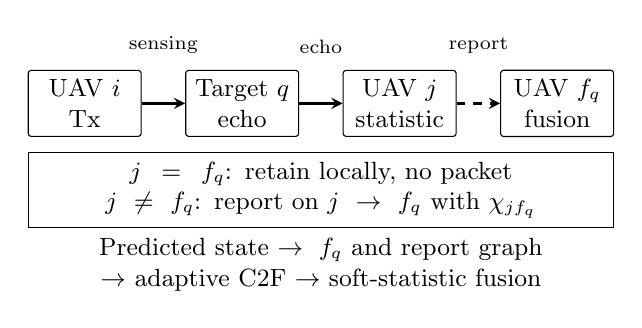
\begin{tikzpicture}[>=stealth, every node/.style={font=\small},
box/.style={draw,rounded corners=1pt,align=center,minimum height=8mm,text width=12mm}]
\node[box] (tx) at (0,0) {UAV $i$\\Tx};
\node[box] (tg) at (2,0) {Target $q$\\echo};
\node[box] (rx) at (4,0) {UAV $j$\\statistic};
\node[box] (fc) at (6,0) {UAV $f_q$\\fusion};
\draw[->,thick] (tx) -- node[above=5mm,font=\scriptsize] {sensing} (tg);
\draw[->,thick] (tg) -- node[above=5mm,font=\scriptsize] {echo} (rx);
\draw[->,thick,dashed] (rx) -- node[above=5mm,font=\scriptsize] {report} (fc);
\node[draw,align=center,text width=72mm] at (3,-1.1)
{$j=f_q$: retain locally, no packet\\
 $j\ne f_q$: report on $j\to f_q$ with $\chi_{jf_q}$};
\node[align=center,text width=72mm] at (3,-2.05)
{Predicted state $\to f_q$ and report graph\\
 $\to$ adaptive C2F $\to$ soft-statistic fusion};
\end{tikzpicture}}
\caption{Sensing and reporting have different endpoints. The fusion UAV is
chosen from predicted target state before observation selection and reporting.}
\label{fig:system_framework}
\end{figure}
